%% AMS-LaTeX Created by Wolfram Mathematica 9.0 : www.wolfram.com

\documentclass{article}
\usepackage{amsmath, amssymb, graphics, setspace}

\newcommand{\mathsym}[1]{{}}
\newcommand{\unicode}[1]{{}}

\newcounter{mathematicapage}
\begin{document}

\begin{doublespace}
\noindent\(\pmb{\text{points}=\text{RandomVariate}[\text{NormalDistribution}[0,1],\{20,1000\}];}\\
\pmb{\text{For}[i=1,i\leq 20,i\text{++},\text{points}[[i]]=\text{points}[[i]]/\text{Norm}[\text{points}[[i]]]*100];}\\
\pmb{\text{getDis}[\text{m$\_$}]\text{:=}\text{Table}[\text{Norm}[m[[i]]-m[[j]]],\{i,1,20\},\{j,1,20\}];}\\
\pmb{\text{proj}[\text{d$\_$}]\text{:=}\text{Table}[\text{If}[j\leq d,\text{points}[[i,j]],0],\{i,1,20\},\{j,1,1000\}];}\\
\pmb{\text{calcError}[\text{m1$\_$},\text{m2$\_$}]\text{:=}\text{Sum}[((\text{m1}[[i,j]]-\text{m2}[[i,j]])/}\\
\pmb{(\text{m1}[[i,j]]+10{}^{\wedge}-20)){}^{\wedge}2,\{i,1,20\},\{j,1,20\}]}\\
\pmb{\text{draw}[\text{m$\_$}]\text{:=}\text{Print}[\text{Histogram}[\text{Flatten}[m],20]]}\\
\pmb{\text{Do}[\text{Print}[\text{calcError}[\text{getDis}[\text{points}]*k/1000,\text{getDis}[\text{proj}[k]]]];}\\
\pmb{\text{draw}[\text{getDis}[\text{proj}[k]]],\{k,\{100,50,10,5,4,3,2,1\}\}]}\)
\end{doublespace}

\noindent\(1692.46\)

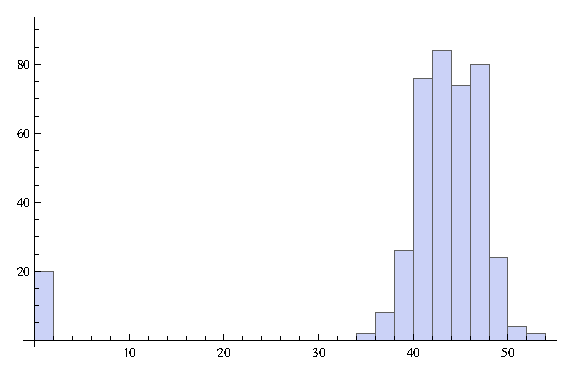
\includegraphics{1_gr1.eps}

\noindent\(4339.74\)

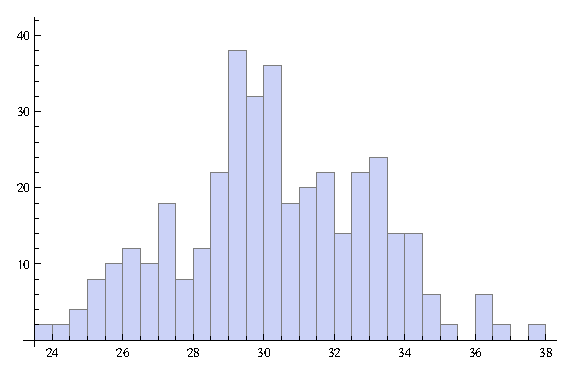
\includegraphics{1_gr2.eps}

\noindent\(33018.2\)

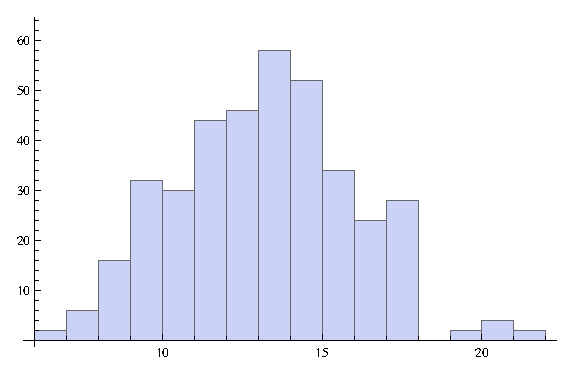
\includegraphics{1_gr3.eps}

\noindent\(56942.4\)

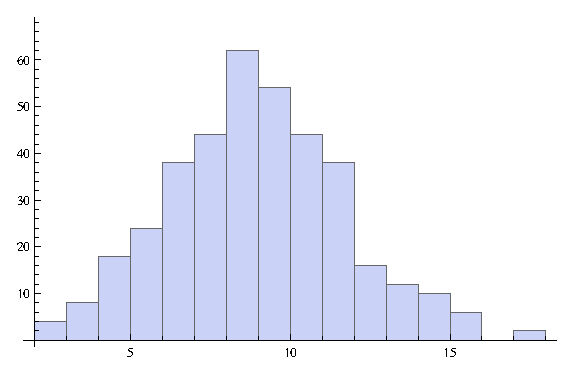
\includegraphics{1_gr4.eps}

\noindent\(79749.\)

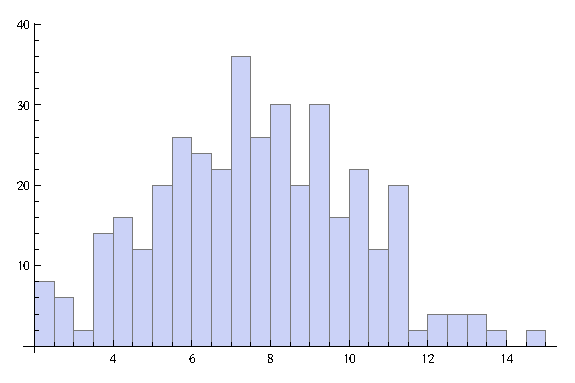
\includegraphics{1_gr5.eps}

\noindent\(118775.\)

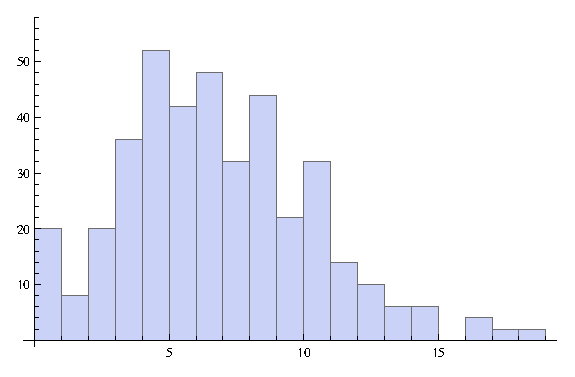
\includegraphics{1_gr6.eps}

\noindent\(191376.\)

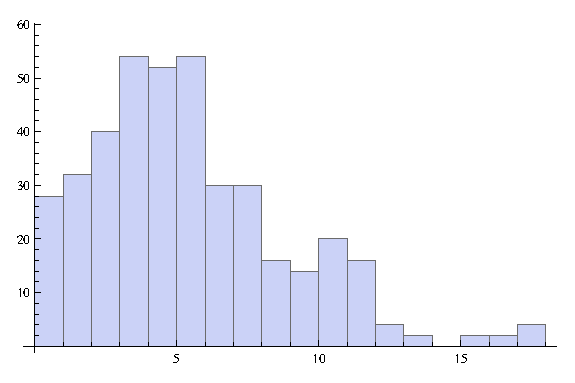
\includegraphics{1_gr7.eps}

\noindent\(378386.\)

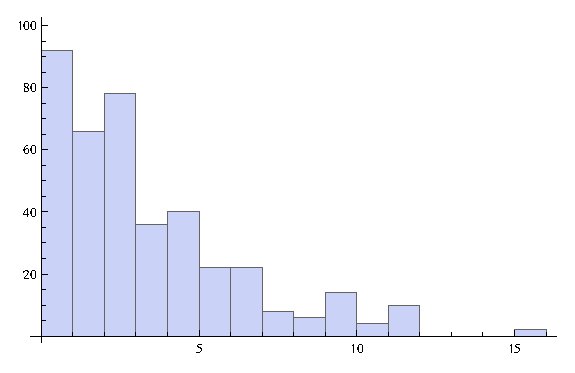
\includegraphics{1_gr8.eps}

\end{document}
